\chapter{Datasets} \label{ch:data_sets}
In this chapter, we provide an overview of the publicly available datasets for the person re-ID. We then describe in details the MARS dataset, which we used in our experiments, together with the cleansing process that we applied to select the most suitable video sequences from all videos of the MARS dataset.
\section{Overview}
There are several publicly available datasets for the person re-ID. A comprehensive overview can be found in \cite{re_ID_data_overview}. One of the first was the ViPeR dataset \cite{ViPeR} released in 2007. It contains 1264 images of 632 identities. Since then, a few more small-scale datasets appeared. The first dataset large enough for deep learning was the CUHK03 \cite{cuhk03} introduced in 2014. It includes 13164 images of 1360 persons. One of the most popular person re-ID datasets is the Market-1501 dataset \cite{market_dataset} from the year 2015. It consists of 12936 images of 751 persons. This dataset was later extended into a MARS dataset \cite{MARS}, which is the first large scale video-based person re-id dataset \cite{re_ID_data_overview}. This dataset was used for our experiments, and we describe it later in this chapter in more details. To my knowledge, the biggest re-ID dataset with respect to the number of identities to date is the MSMT17 dataset \cite{MSMT17}. It consists of 4101 identities and 126441 images. This dataset, however, does not contain tracking sequences and could not have been used for our purposes.
\section{MARS Dataset}
For the purpose of this thesis, we have used the MARS dataset \cite{MARS}, which is the biggest video-based person re-ID dataset to date \cite{re_ID_data_overview}. It contains 1261 identities and 1191003 video frames from around 20715 videos. All the recorded videos come from six near-synchronized cameras in the campus of Tsinghua. An example of a video sequence consisting of seven image frames is displayed in Figure
\ref{fig:mars_example}.

\begin{figure}[h!]
    \centering
    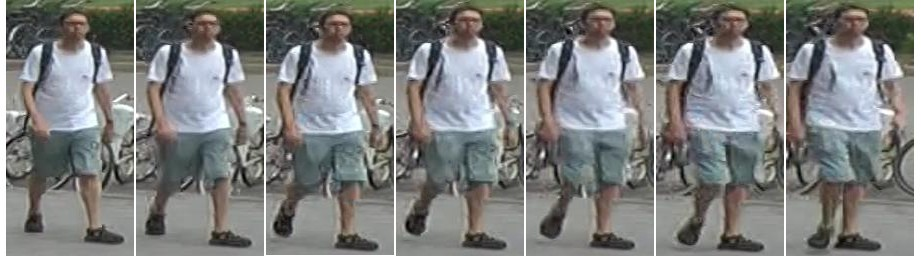
\includegraphics[scale=0.4]{figures/0006C2T0002F016_22.jpg}
    \caption{MARS data set example} 
    \label{fig:mars_example}
\end{figure}


Even though MARS dataset is a suitable dataset to be used as a training dataset for the person re-identification from video, there are some issues which have to be solved before using it for the model training. 

\subsection{Issues of the data set in re-ID}

The main problem of the raw dataset is the so called Class Imbalance Problem \cite{class_imbalance}, which in case of the MARS data set means that the number of video sequences per identity varies significantly, ranging from 1 to 271 videos. Hence, when training a classification model, the identities for which there are many video sequences in the training dataset would be prioritized by the model which would harm its generalization ability. 

Another issue is the length of the videos, which ranges from very short sequences consisting of less than five image frames up to very long sequences depicting dozens of steps of a walking person. If we want to build a model that should re-identify an identity based on the way they walk, the very short videos will not provide enough information for the model to be able to recognize them.

The third problem that needs to be mentioned when talking about the MARS dataset is the quality of the videos, which is also varying throughout the dataset. The most frequent defect of the videos is the partial occlusion, which limits the possibility to describe the movement of the whole bodies.

\subsection{Dataset cleansing} \label{dataset:cleansing}
In order to solve the previously mentioned issues, we apply the following cleansing process on the MARS dataset. We cut the original video sequences into subsequences of 20 images, which roughly corresponds to a video of two steps of a walking person. The reason why we decided for the sequences of 20 images is that even though we would extract more information about the identities from longer sequences, we would loose a lot of identities as for many of them, there is not enough data to extract sufficient amount of longer video sequences. From these short sequences, we select up to 10 sequences for each identity. The selection is based on a parameter that denotes the quality of the sequence with respect to visibility of the moving identity. This step will be further explained in Chapter \ref{ch:proposed_solutions}. Out of these ten sequences, at most 4 come from the same camera as such video sequences are very similar and would not bring any additional value for the model training. Those identities where there are less than 4 such video cuts are dropped from the data set. This way, we obtain a data set consisting of 1210 identities. The distribution of number of identities for number of videos is displayed in diagram \ref{fig:num_of_videos_per_id}.

\begin{figure}[h!]
    \centering
    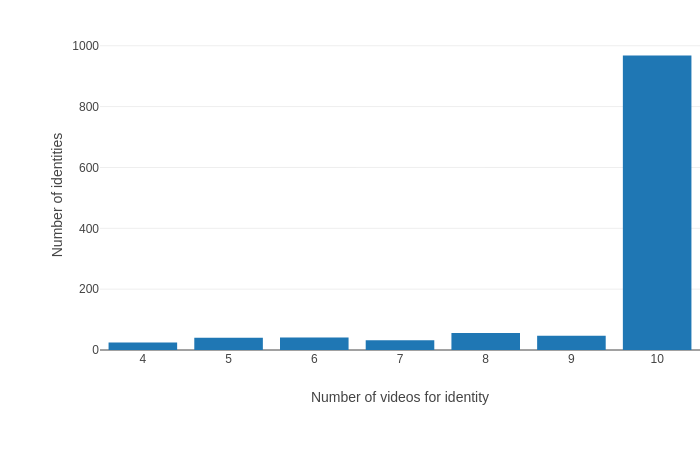
\includegraphics[scale=0.4]{figures/identities_per_num_of_videos.png}
    \caption{Distribution of number of identities for number of videos} 
    \label{fig:num_of_videos_per_id}
\end{figure}


